\documentclass[12pt,letterpaper]{article}

\usepackage[utf8]{inputenc}
\usepackage[T1]{fontenc}
\usepackage{amsmath}
\usepackage{amsfonts}
\usepackage{amssymb}
\usepackage{amsthm}
\usepackage[left=2cm,right=2cm,top=2cm,bottom=2cm,headheight=22pt]{geometry}
\usepackage{fancyhdr}
\usepackage{setspace}
\usepackage{lastpage}
\usepackage{graphicx}
\usepackage{caption}
\usepackage{subcaption}
\usepackage{paralist}
\usepackage{url}

\theoremstyle{definition}
\newtheorem{question}{Question}
\newtheorem{example}{Example}
\newtheorem{exercise}[question]{Exercise}
\newtheorem*{challenge}{Challenge}
\newtheorem*{theorem}{Theorem}
\newtheorem*{definition}{Definition}

\begin{document}

%Paramètres de mise en forme des paragraphes selon les normes françaises
\setlength{\parskip}{1ex plus 0.5ex minus 0.2ex}
\setlength{\parindent}{0pt}

%Paramètres relatifs aux en-têtes et pieds de page.
\pagestyle{fancy}
\lhead{Theron J Hitchman}
\chead{\Large Reading and Guided Practice \#07}
\rhead{Spring 2016}
\lfoot{\emph{Math and Decision Making }}
\cfoot{}
\rfoot{\emph{\thepage\ of \pageref{LastPage}}}

\section*{Introduction}

In this reading, you will learn the basics of a fun new way to tell graphs apart, using colors!

\section*{Goals}
At the end of this assignment, a student should be able to:
\begin{compactitem}
\item state and use the definition of an $n$-coloring of a graph,
\item decide if simple graphs have an $n$-coloring, for a particular value of $n$, and
\item find the chromatic number of some simple graphs.
\end{compactitem}
A student might also be able to:
\begin{compactitem}
\item Solve a challenging puzzle about the chromatic number of planar graphs.
\end{compactitem}

\section*{Reading and Questions for Graphs Day 08}

\begin{exercise}
Get some colored pencils or some crayons to supplement your usual writing instrument. Draw a graph with
your regular pen or pencil. Make sure your graph has lots of vertices. Now, here's the fun part. Use your colored
pencils and crayons to color in all of the vertices. WAIT! There is a rule: If two vertices are joined with an edge
(graph theorists say they are \emph{adjacent} vertices), then those vertices must be different colors.
Can you do it? 

Take a minute and try.
\end{exercise}


Fix a number $n$. (If you like, imagine the number is $n=4$). An $n$-coloring of a graph is a labeling of the vertices
of the graph so that each vertex gets a color, and each pair of adjacent vertices get different colors.

\begin{figure}[h]
\centering
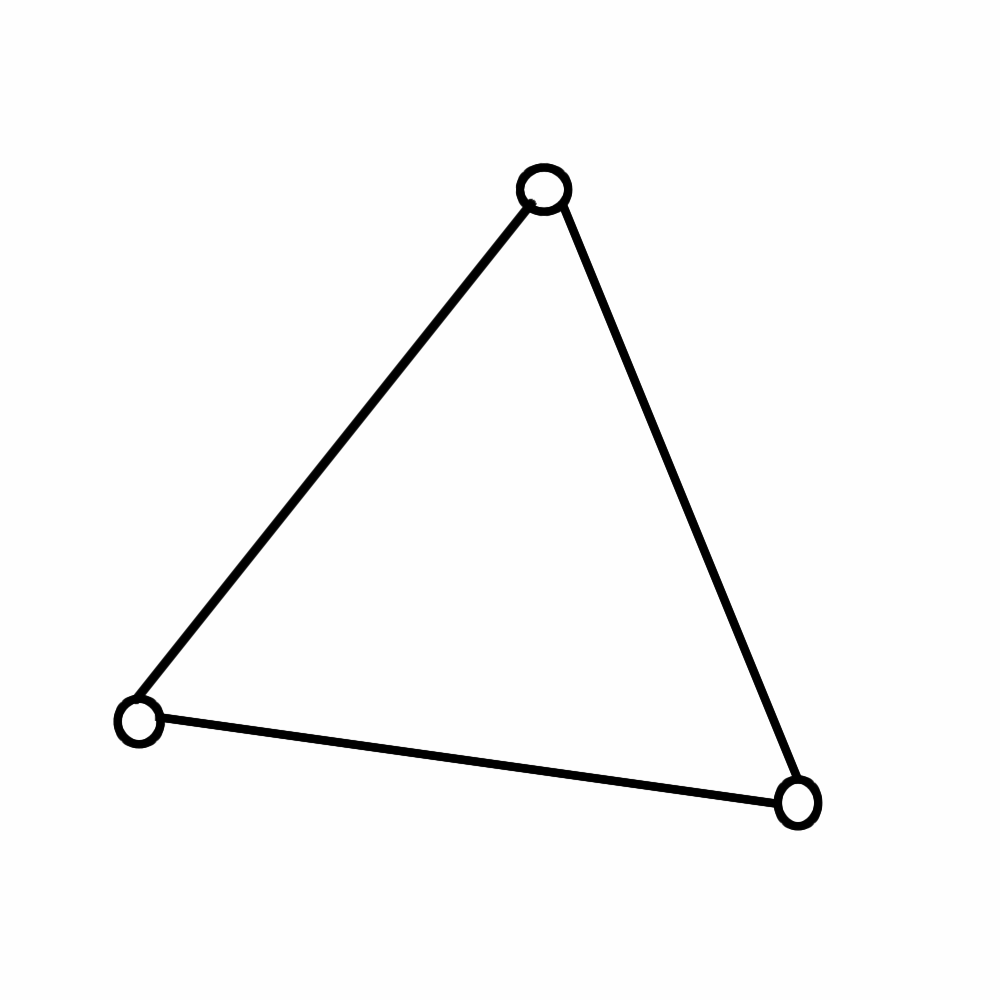
\includegraphics[width=.3\textwidth]{images/k3.png}
\caption{The graph $K_3$ is a triangle}
\label{fig:k3}
\end{figure}

For example, the complete graph on 3 vertices is a triangle, and it has a $3$-coloring. Just put a different color 
on each of the three vertices.

The graph which is just a simple cycle and can be given a $2$-coloring.
\begin{figure}[h]
\centering
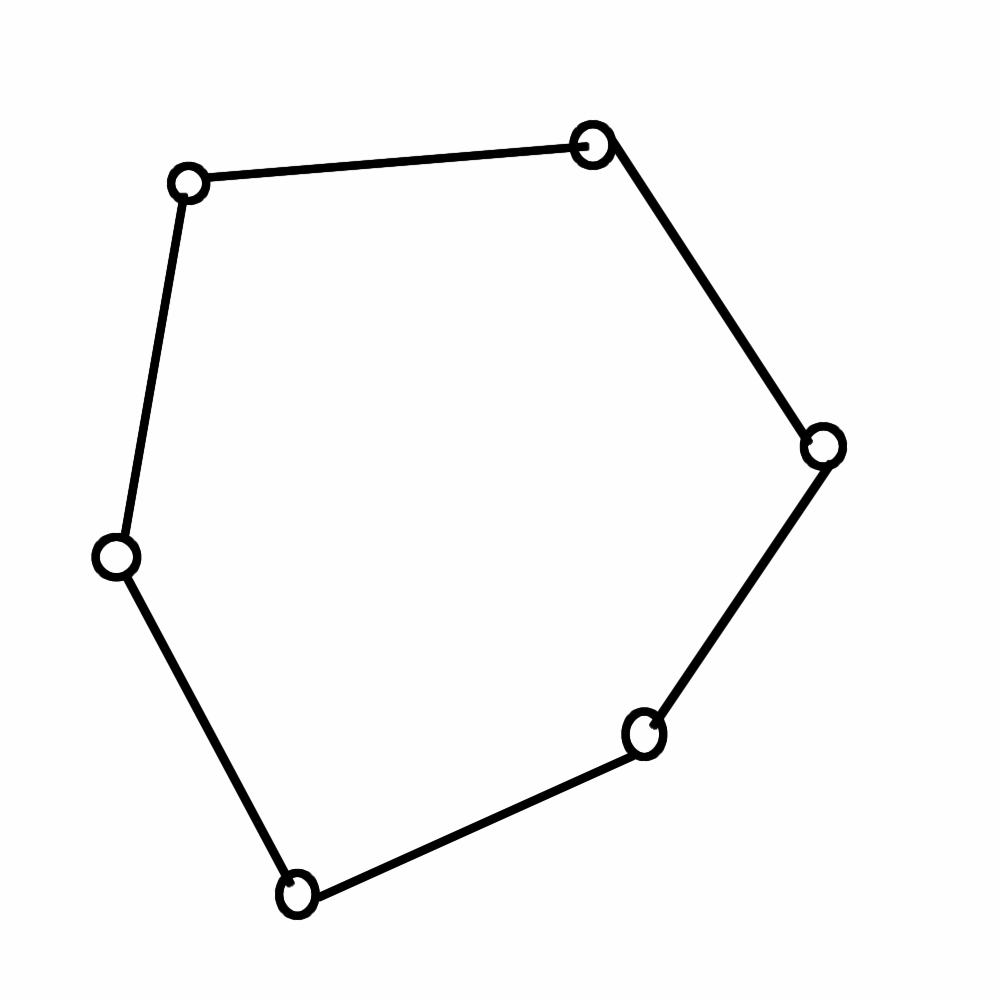
\includegraphics[width=.3\textwidth]{images/cycle.png}
\caption{A graph consisting of a single simple cycle}
\label{fig:cycle}
\end{figure}

\begin{exercise}\label{ex:2color}
Find a $2$-coloring of the graph in Figure \ref{fig:cycle}.
\end{exercise}

\begin{exercise}\label{ex:3color}
Can the graph in Figure \ref{fig:cycle} be given a $3$-coloring?
\end{exercise}

Here is a sticky point: the rules for making an $n$-coloring do not \emph{require} that all $n$ colors get used!
So, the graph in Figure \ref{fig:cycle} has a $5$-coloring. You already made one in Exercise \ref{ex:2color}, and 
you looked for another in Exercise \ref{ex:3color}. Just because there weren't exactly 5 colors doesn't cause a 
problem.

\begin{exercise}
Find a $4$-coloring of the Three Utilities Graph $K_{3,3}$.
\end{exercise}

\begin{figure}[h]
\centering
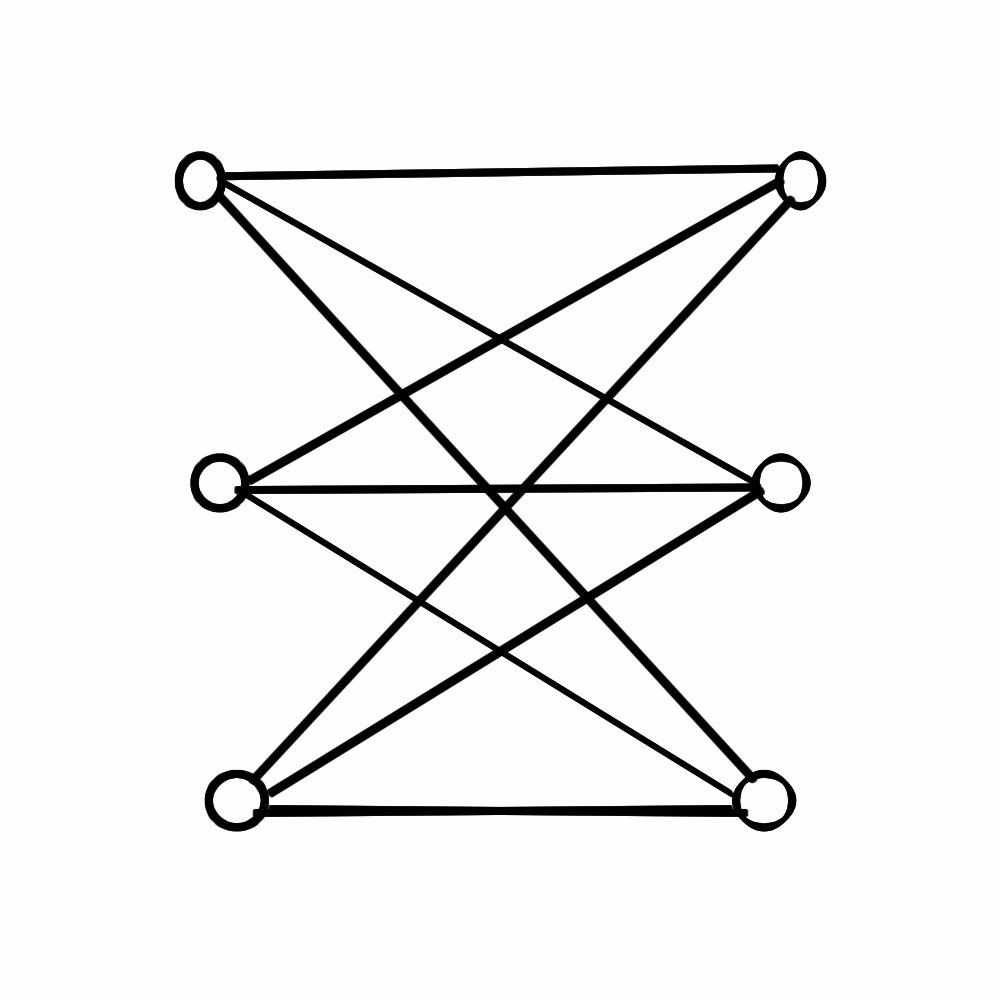
\includegraphics[width=.3\textwidth]{images/k3,3.png}
\caption{The graph $K_{3,3}$}
\label{figure:k33}
\end{figure}


\subsection*{What Do We Get From This?}

First of all, playing with colored pencils is fun and soothing. Don't forget that.

The ability to find an $n$-coloring for a particular value of $n$ is an \emph{invariant}. If you have a pair of graphs
$G$ and $G'$ and they are isomorphic, then the correspondence between the two graphs will allow you to carry
a pattern of colors from one to the other.

But this gets \emph{used} in the other direction. If $G$ has an $n$-coloring, but $G'$ doesn't have an $n$-coloring, 
then those graphs cannot be isomorphic! We get another nice way to say for sure that two graphs are truly different.

\begin{exercise}
Use the idea of ``having an $n$-coloring'' to say why you know that the graph $K_{3,3}$ and the graph $K_6$ are
not isomorphic.
\end{exercise}


\subsection*{The Chromatic Number}

We can use $n$-colorings in a more refined way. When you do it like this you sip your tea with your pinkie sticking straight out. (No slurping!)

The \emph{chromatic number} of a graph is the smallest value of $n$ so that the graph has an $n$-coloring. 
There is notation for this that mathematicians use. We write $\mathrm{chr}(G) = k$ when the chromatic number
of $G$ is equal to $k$.

For example, our triangle graph $K_3$ has no $1$-coloring and it has no $2$-coloring. But it does have a $3$ coloring. So we say that the chromatic number of $K_3$ is equal to $3$.

\begin{exercise}
Check the claims in the last three sentences. There are four things to do.

When you are done, you should be sure that $\mathrm{chr}(K_3) = 3$.
\end{exercise}


\subsection*{Challenge}

Find a map of the State of Iowa which shows all of the counties and their boundaries. Iowa has 99 counties, so the 
map is a little intense. You want to color the map in so each county is one solid color, and two counties
which share a boundary have different colors.

How many colors do you need? Can you do it with five colors? With four?



%\begin{thebibliography}{9}
%\end{thebibliography}

\end{document}
%sagemathcloud={"zoom_width":100}